\documentclass[twocolumn,11pt,english]{article}
\usepackage{listings}
\usepackage{amsmath}
\usepackage{amsfonts}
\usepackage{cite}
\usepackage[T1]{fontenc}
\usepackage{graphicx}
\usepackage{color}
\usepackage{verbatim}
\usepackage[margin=1.0in]{geometry}
\lstset{language=Haskell}

\addtolength{\topmargin}{-0.5in}

\title{Maybe Slipstreams}
\date{}
\author{
  Carlyle, John\\
  \textit{jcarlyle@ucsc.edu}
  \and
  McDermott, Morgan\\
  \textit{mmcdermo@ucsc.edu}
}


\begin{document}
\maketitle

\section*{Abstract}
We give a definition of \textit{Functional Reactive Programming} (FRP) that allows for dynamic signal networks and safe interaction with the real world. We allow signal networks to be dynamic by modeling them as higher-order streams (as in Patai \cite{HighOrderStreams}), and use the concept of wormholes (from Winograd \cite{WinogradCort2012HS}) to make interaction with real world resources safe. All signal values are modeled as $Maybe$ values to allow for defined behavior in the face of disrupted signals, and to reference signal values before they have any reasonable value. We also specify a DSL that uses this FRP model, allowing a programmer to easily design signal networks to accomplish tasks by specifying layers and how the layers interact. Our implementation builds on previous work by being more practical. The DSL arises naturally from our definition of FRP, is simple to use and requires only limited knowledge of the underlying FRP concepts.

\section{Introduction}
  
Functional Reactive Programming, introduced by Fran \cite{ElliottHudak97:Fran}, is a programming paradigm allowing for the manipulation of time-varying values with pure functions. Fran was declarative, allowing the programmer to express the ``what'' of a program with interconnected time-varying values, which implies ``how'' the program should be instantiated. 

The original implementations of FRP like Fran divided time-varying values into two types: \textit{Events}, or a discrete stream of values modeled by $Event~a:: [a]$, and \textit{Behaviors}, or continuous functions of time modeled as $Behavior~a :: t \rightarrow a$. 

Behaviors are always implemented by sampling their value at chosen intervals, since computers perform discrete operations. The advantage of behaviors is that their resolution is arbitrary - they have a precise value whenever they are sampled. With a low enough sample, rate a behavior could be considered an Event, but generally Events are used to model things that are truly discrete (like mouse clicks), etc. 

These first FRP systems allowed the programmer to express higher-order FRP constructs, like Behaviors of Behaviors, but in so doing allowed the user to inadvertently create time and space leaks. 

In FRP, it is possible to depend on values that are far in the past. Clearly, the longer the program is executing, the longer the history of events. If the composition of FRP constructs depends on past values, we accumulate a longer stream that takes up more memory and can cause slowdown if the stream is not trimmed after a certain point. 

Consider the function $integral$, that takes a Behavior and integrates over all of its past values. 
\begin{align*}
  integral :: Behavior~Int \rightarrow Behavior~Int
\end{align*}
If we have higher-order constructs, it would be possible to first calculate this integral at a time $t > 0$ - this would require, however, calculating the initial behavior at all sample times from $0 < t_{sample} < t$. 

It is also challenging to determine when past values will never be used. Typically a garbage collection service is used to clean up old events which are no longer dependencies. This is analogous to a memory leak in imperative programming. Similarly, values are often unnecessarily preserved in memory despite not being used in any current computation. 

\subsection{Why use FRP}
 The complexity of modern GUI (Graphical User Interface) code motivates our development of this system. FRP is a useful approach to user interface design because it permits the user to declaratively describe the complex interaction between GUI elements. Using imperative programming, GUI design is often achieved with callbacks and notifications about interaction events. 

The common approach leads to extremely messy user interface code, often dubbed ``callback hell'' in the context of javascript \cite{czaplicki2013asynchronous}.. 
Using time varying values in an FRP network, the programmer can describe \textit{what} an interface element is rather than how it responds to and changes the environment. The user can compose these elements together to achieve a declarative description of the user interface. From this structure, the relationship between pieces of the interface implicitly emerges, freeing the programmer from having to tediously define exactly how each relationship is enacted.

\subsection{Problems with FRP}
  Current FRP systems have several drawbacks. In order to avoid time and space leaks, Yampa \cite{hudak2003arrows} introduces arrowized FRP. The security is provided by not making FRP constructs first-class. Instead of Behaviors and Events, arrowized FRP uses $Signal$s, which take on the type of behaviors:
\begin{center}
  $Signal~a:: t \rightarrow a$
\\$SF~a~b:: Signal~a \rightarrow Signal~b$
\end{center}

Signals are not first class in arrowized FRP, however. The basis of arrowized FRP interface is the $Signal~Function$, referred to by the type $SF~a~b$. This system then uses the well understood $Arrow$ structure to compose Signal Functions and create a sort of network of transformation. 

The problem with arrowized FRP is that it has a limited ability to express dynamic networks of signal functions. In Yampa there are $switch$es that given two signals can choose one of them to output at any given time. This, however, is far from the dynamism we need to implement certain GUI constructs. 

 In our system, we solve the problem of having first class FRP constructs by using a modified stream-based FRP model\cite{HighOrderStreams}, to obtain the safety of Arrowized FRP and the expressiveness of classical FRP. A stream is essentially a complete history of the values of a particular computation. Any other computation that needs the current value, or a value from the past, can look at the stream and find the appropriate values. This leads to additional problems like memory usage growing out of control as new values are continually added to the stream and not removed. In some systems garbage collection finds and removes values from streams that are no longer dependencies for other computations. In Elerea \cite{HighOrderStreams}, this is solved by only allowing access to the most recent values in streams. 


\subsection{Organization}
This paper primarily introduces a way for FRP to interact safely in an environment filled with hazerdous resources which are difficult to model as a function of time. (What the different sections are for) (Section 1) Section 2 Section 3 Section 4 Section 5 Section 6 Section 7.

\section{A Motivating Example}
Our goal is to adapt FRP for javascript GUI development, avoiding the horrors of \textit{callback hell}. One particular problem that often results in mangled code is asynchronous communication between a server and client through AJAX. In our model, we can think of both the discrete values being sent to the server, and the discrete values being received, as a time-varying value sampled at an appropriate interval. 

In order to model this situation we need to augment stream basd FRP. Streams need to interact with the environment in a safe way. For example streams also need to be able to model asynchronous requests.

We need to model the changing requirements for interfaces. If the user presses a button to submit a query to the server, the server could respond by indicating that interface on the page should be fundamentally changed. Perhaps we need to create more buttons that could perform different server queries, or remove some functionality from the GUI. In order to solve this, we need a dynamic FRP network that can modify itself. 

Classical FRP and Elerea are capable of modeling this situation since they have first-order FRP constructs. In our case we would use Elerea's solution of higher-order streams to implement this use case. 

We need to ensure that the time-based values from the server are treated in a well-defined way. Namely, what if we have never contacted the server? What should the value of its stream be, and how should that differ from the stream after it has responded and is in an idle state again? We solve this problem by encapsulating every stream value in a $Maybe$, as we will explain later. 

Lastly, what happens when two computations wish to change the state of the interface at the same time? How can we allow safe interaction between external state and multiple effectful FRP functions that wish to modify the same state? We solve this using Wormholes as defined by Winograd-Cort \cite{WinogradCort2012HS}.

\section{Network Dynamism through Higher Order Streams}
In order to express the dynamic behavior that we need to implement GUIs, the underlying signal network needs to be able to change itself over time. We choose to model this dynamism with higher order streams like Patai\cite{HighOrderStreams}. This method avoids the time and space leaks that were present in other FRP systems with first class signals/behaviors/events \cite{ElliottHudak97:Fran}. 

Patai defines his model in terms of \textit{Denotational Design} developed by Conal Elliot \cite{elliott2009denotational}. The core idea Patai leverages is the \textit{Type Class Morphism}, or defining an interface by a combination of its \textit{type} and its \textit{properties}. By focusing on the interface, this design strategy allows implementations to be checked for correctness but to otherwise have freedom in their methodology. 

The core type in Patai's stream model is \textit{Stream a}, representing a stream of values over time. This is analagous to a Behavior, and in fact has the same type signature: 
\begin{equation}
  \textbf{type}~\textit{Stream a} = \mathbb{N} \rightarrow a
\end{equation}
Any  s::\textit{Stream a} can be thought of as the stream of values:
\begin{equation}
  \langle s_0 s_1 s_2 ... s_n \rangle ~where~ s_i :: a
\end{equation}
Patai makes Stream take on the Monad and Applicative typeclass interfaces, following the strategy of Denotational Design. Initially Patai models these Streams using a \textit{cons} constructor that represents a delay of one timestep. However, if we use this stream definition and consider a higher order stream of type \textit{Stream (Stream a)}, we end up with quadratic performance for \textit{join} when we attempt to extract a value from the \textit{Stream (Stream a)}. This is fairly obvious if we try to visualize the higher order stream, since the values of $join~s$ where $s$ :: \textit{Stream (Stream a)} are the main diagonal of the stream of streams:

\begin{align*}
    \langle &\langle \mathbf{v_{00}} ~ v_{01} ~ v_{02} ~ ... ~ \rangle \\
    &\langle v_{10} ~ \mathbf{v_{11}} ~ v_{12} ~ ... ~ \rangle \\
    &\langle v_{20} ~ v_{21} ~ \mathbf{v_{22}} ~  ...  ~ \rangle \rangle
\end{align*}

To solve this problem, Patai moves away from the \textit{cons} definition of Streams. Instead, he creates streams and higher order streams from three primitives: $delay$, $start$, and $generator$. He also introduces the type $StreamGen$, which has the same signature as a $Stream$ but is only used to represent higher order streams. 

\small
\begin{equation}
  \mathbf{type}~\mathit{StreamGen~a} = \mathbb{N} \rightarrow a
\end{equation}
\normalsize
The $delay$ function replaces cons in this new configuration. The difference is that instead of returning a $Stream$, it returns a $StreamGen$. It functions by returning its first argument at $t = 0$, and the first $Stream~a$ applied to the sample time otherwise. For intuition, we've also included the simplified type:
\small
\begin{align*}
dela&y :: a \rightarrow Stream~a \rightarrow StreamGen~(Stream~a)\\
dela&y :: a \rightarrow (\mathbb{N} \rightarrow a) \rightarrow (\mathbb{N} \rightarrow~(\mathbb{N} \rightarrow~a))\\
dela&y~x~s~t_{start}~t_{sample} =\\
&|~t_{start} = t_{sample} = x\\
&|~t_{start} < t_{sample} = s (t_{sample} - 1)\\
&|~otherwise ~~~~~~=\perp
\end{align*}
\normalsize

The $start$ function simply gives us a safe way to extract a stream from a stream generator. Given that $delay$ is undefined if $t_{start} > t_{sample}$, a universally safe time for $t_{start}$ is 0.
\small
\begin{align*}
&start :: StreamGen (Stream~a) \rightarrow Stream a\\
&start g = g~0
\end{align*}
\normalsize

However, given $t_{sample}$ there is another safe value: $t_{start} = t_{sample}$. This concept is embodied in the function $generator$: 
\small
\begin{align*}
&generator :: Stream~ (StreamGen a) \rightarrow Stream~a\\
&generator~g~t_{sample} = g~t_{sample}~t_{sample}
\end{align*}
\normalsize
\begin{comment}
TODO: DISCUSS THE FANCY EFFICIENCIES AND BIND AND JOIN ETC
\begin{align*}
  \langle &\langle \mathbf{v_{00}} ~ v_{01} ~ v_{02} ~ v_{03} ~ ... ~ \rangle \\
  &\langle \perp ~ \mathbf{v_{11}} ~ v_{12} ~ v_{13} ~... ~ \rangle \\
  &\langle \perp ~ \perp ~ \mathbf{v_{22}} ~ v_{23} ~ ...  ~ \rangle \rangle
\end{align*}


Better idea to avoid wasted space and complex ge


\begin{align*}
  \langle &\langle \mathbf{v_{00}} ~ v_{01} ~ v_{02} ~ v_{03} ~ ... ~ \rangle \\
  &\langle  \mathbf{v_{11}} ~ v_{12} ~ v_{13} ~ v_{14} ~ ... ~ \rangle \\
  &\langle  \mathbf{v_{22}} ~ v_{23} ~ v_{24} ~ v_{25} ~ ...  ~ \rangle \rangle
\end{align*}
\end{comment}

\subsection{Application of the stream model}
Patai modifies his definition of a stream to $Stream~a :: IO a$ in his implementation, since the time index is implicit. Likewise in our model we do not explicitly model time for $Signal$s, and allow Signal Functions to be effectful. 

Our $Signal$ Monad fulfills the requirements for $Stream$s: extracting a value from the monad is idempotent (will always produce the same sampled value during the same timestep), and is commutative (the order in which $Signal$s are sampled does not matter). 

We avoid space-time leaks just as Elerea does, by disallowing access to previous values of Streams/Signals (and implicitly starting newly created streams at a local time of 0, rather than trying to ``catch up'' with global time). 

Unlke Elerea, we do not use $delay$ as a base primitive, instead using $foldp$ as a means of delaying signals to create new signals. 


\section{Real World Interfaces}
\subsection{Signals as Maybe Streams}
  Consider modeling a stream of data from a server to a browser GUI. There are two situations when the value of this stream might have an undefined value: If the connection between server and browser has not yet been initiated, or if it has been disrupted. 

To model the two cases of \textit{disruption} and \textit{pre-existence}, we introduce what we're calling a $Signal$, which is roughly modeled as:
\begin{equation}
  \textbf{type}~\textit{Signal a} = Stream (Maybe~a)
\end{equation}
At any point in time, a $Signal$ may now be defined but have a $Nothing$ value. We can now be assured that any system behavior dependent on this value will act in a defined way even given possible disruption. 

As in the given motivating example, we could now also reference the current value of a stream of data coming from the server before we ever initiate the connection.

\subsection{Resources and Wormholes}
If Signal Functions are allowed to be effectful, the side effects of evaluating an FRP network can be hard to determine. Since the values of Signals are sampled at an interval, the difficulty of understanding the effects of the effectful signal functions is further compounded. 

Consider the example given by Winograd-Cort\cite{WinogradCort2012HS} - if we have two signal functions that send a value to a speaker, then both get evaluated at every sampling of the signal network. The value of the speaker is then dependent on the order of evaluation of signal function nodes in the network, which should be hidden from the user. 

To solve this problem, Winograd-Cort introduces \textit{Resource Types} and \textit{Wormholes}. Resource Types are a phantom type parameter associated with all signal functions. If a signal function interacts with a resource, that resource is added to the set of resource types in its type. To compose two signal functions, then, their sets of resources must be disjoint. 

This means that two signal functions can only be composed if they don't access any of the same resources. This idea of restricting access to physical resources is extended to ``virtual resources'' (values in memory) with the concept of \textit{Wormholes}. A Wormhole consists of a Blackhole, into which data may be written, and an associated Whitehole, out of which data may be read. 

Since this effectively gives the user mutable memory, in order to keep the meaning of programs clear, resource types are used to ensure that no two composed signal functions write to the same Blackhole. 

\subsection{Implementing Safe Resources}
In our FRP system, management of resource types is given to low-level libraries. We model both wormholes and access to physical resources as effectful signal functions - that is, sending input to an effectful signal function is equivilant to sending information to a blackhole, and extracting information from it is equivilant to extracting information from a whitehole.

To interact with a speaker, we could have the following effectful Signal Function:
\small
\begin{align*}
  speakerValue~::~SpeakerID \rightarrow SF~Value~Value
\end{align*}
\normalsize

The function $speakerValue$ would return a signal function of type $SF~Value~Value$ tagged by the resource type $Speaker \times \{SpeakerID\}$. 

This tag only restricts what functions may be composed with speakerValue ($f \circ speakerValue~ID$), and not what functions speakerValue may be composed with ($speakerValue~ID \circ f$).

Since our FRP system will not be implemented in an environment with a strong type system, resource types are checked at runtime during signal function composition (But before evaluation of the signal network). 

\section{DSL}

A major roadblock in FRP adoption is its complexity. Understandably, FRP implementations attempt to be as expressive as possible. Our implementation, for example, extended the basic idea of Elerea and Elm with additional safety measures for real world interaction. 

The goal of our DSL is to bridge the gap between a complex, fully expressive FRP system, and something that can be easily used to express a usable FRP program. It is intended to rest atop more complicated FRP libraries, enabling access for a new class of end users who want a quick and intuitive interface.

Because of this, our DSL does not directly permit the user to create effectful signal functions tagged with resource types. Instead, the user can use a number of precreated libraries, or create their own library and use the DSL atop their implementation. 

\subsection{DSL Components}

When implementing software with FRP, dependencies between values can be confusing. This is why in our DSL, we restrict dependencies by dividing Signal values into \textit{layers}. Layers are composed of \textit{elements}, representing time-varying values ($Signal$s) computed from previous values. To maintain the desired ease of understanding, elements can only depend on the values of elements from the previous layer. 

\begin{figure}[h!]
  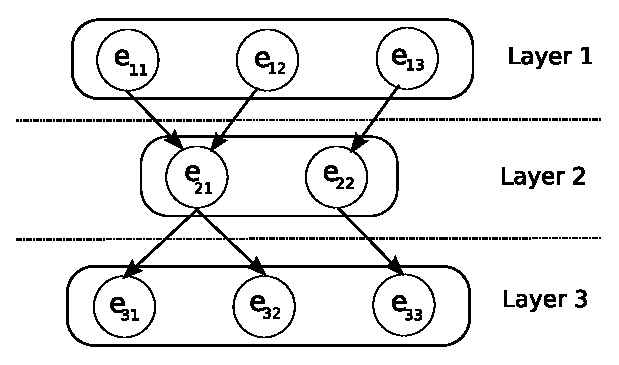
\includegraphics[scale=0.8]{layers.eps}
\caption{DSL Layers and Elements}
\label{fig:layers}
\end{figure}

In Figure~\ref{fig:layers}, arrows represent dependencies. Element $e_{22}$, for example, depends on $e_{11}$ and $e_{12}$. In this system, the output of the FRP program is defined as the tuple of the values of the elements of the last layer; The output of this FRP program would be $(e_{31}, e_{32}, e_{33})$.

\begin{comment}
\begin{description}
\item[behavior] Using the previous definition of an element and a signal, an element can be thought of as a function that maps from one signal to another. More concretely \\
  $type~element~a~b = Signal ~a \rightarrow Signal ~b$\\
  Behaviors are typically thought of in terms of continuous functions. What FRP is trying to do is model the change in behavior of some element in a network. This takes up a lot of processor power  and is not very efficient.

\item[event] An event is a discrete behavior. Since behaviors perform so poorly, it is often necessary to break a signal into a set of discrete values. The cutoff is not clear between high and low sampling rates. With a high sample rate, something can be considered a behavior; with a low sample rate it can be considered an event. Our implementation of FRP is skewed toward events.

\item[signal] It is useful to think of the values being sent from one element to another as a signal being broadcast continuously. The element receiving this signal adjusts its own outgoing signal according to a predefined set of rules or a function.

\item[stream] An element may have need of signals from more than one timestep in the past. A stream is essentially a history of all previous values of a signal, with the most current signal value at the head of the list. Streams travel between elements, thus allowing an element to select what timestep it selects a value from. The downside of streams is that they allow for spacetime leaks, which are described below. A stream of type $Stream~a$ will be denoted as $\langle v_0~v_1~v_2~...\rangle$ where $v_i$ is of type $
a$.
\end{description}
\end{comment}
\subsection{DSL Definitions}
\begin{description}

\item[element] Any time-varying value, or any computation that relies upon previous computations or values. An element is essentially a Signal Function that has arity from 0 to $n$ where $n$ is the size of the previous layer. All elements connected to element $e$ can be split into two sets: $s_1$ (all elements supplying input to $e$) and $s_2$ (all elements recieving their input from $e$). $s_1$ is called the predecessor set of $e$ or $s_1 = pred(e)$, and $s_2$ is the successor set of $e$ or $s_2 = succ(e)$

\item[network] A set of elements that form a connected component. Multiple networks can be used to describe different unrelated components of a particular interface or problem space.

\item[layer] A layer is a set of elements in a network where the intersection of their mutual union of predecessor and successor sets is the empty set. More formally,
\begin{equation}
  \bigcup_{e_i \in L}{pred(e_i)} \cap \bigcup_{e_j \in L}{succ(e_j)} = \emptyset
\end{equation}
where $L$ is a layer. Breaking a network into layers is helpful because it helps identify dependencies in the network. It also helps introduce structure into the environment, which can help organize a network during its development. 

\end{description}

The DSL defined in this way cannot express many network topologies. For example, it cannot express feedback loops, and has no way of passing a result back to a predecessor. This technique is useful for maintaining state in a network. As we will show, our DSL provides builtin primitives to enable these behaviors. 

\subsection{DSL Examples}
The goal of the DSL is to easily express \textit{networks} as we've defined them. To express the network from Figure~\ref{fig:layers}, we would write:
\begin{center}
$(e_{11}, e_{12}, e_{13})$
\\ $\rightarrow (e_{21}, e_{22})$
\\ $\rightarrow (e_{31}, e_{32}, e_{33})$
\end{center}
The elements in layer 1 represent functions of type $() \rightarrow Signal~a$, while the elements in all other layers represent a signal function of any arity, i.e.) $Signal~(a, b, ... n) \rightarrow Signal~z$

A program in the actual DSL would therefore have $source$s in the first layer and signal functions or sources elsewhere. Builtin functions of type $() \rightarrow Signal~a$ are prefixed by $@$ in our DSL for clarity. 

In our DSL, $L[expr]$ represents the lifting of an anonymous function that takes as arguments the values of all elements in the previous layer, and whose body is $expr$. That is, 
\begin{center}
$L[\$1 * \$2] \equiv lift (\backslash \$1 ~\$2 \rightarrow \$1 * \$2)$
\end{center}
Using these constructs, a specific network with the same topology as Figure~\ref{fig:layers} might be:
\begin{center}
$(@mousePosX, @mousePosY, @time)$
\\ $\rightarrow (L[sum(\$1, \$2)], L[\$3 * 2])$
\\ $\rightarrow (L[\$1 / 2], L[\$1], L[\$3])$
\end{center}
\subsection{DSL Grammar}
\footnotesize
\begin{align*}
  Statement ::=& ~V \leftarrow Expression &\text{Variable assignment}\\
  |& ~Expression &\text{Single expression}\\
  Expression ::=& ~SignalNet &\text{A signal network}\\
  |& SimpleExpr &\text{An expression}\\
  SignalNet ::=& ~( Exprs ) \rightarrow SignalNet &\text{Compose layers}\\
   |& ~(Exprs ) &\text{Single layer} \\
  Exprs ::=& ~SimpleExpr ~,~ Exprs &\text{List of expressions}\\
  |& ~SimpleExpr &\text{Single expression}\\
  SimpleExpr ::=& ~L[Expr] &\text{Lift}\\
  |& ~ @V &\text{$SF :: () \rightarrow Signal~a$}\\
  |& ~ (V, V) &\text{Tuple}\\
  |& ~ V( Exprs ) &\text{Function call}\\
  |& ~ foldp( @V, V, [Expr] ) &\text{Past-Dependent Signal}\\
  |& ~ Aggregator &\text{New Aggregator}\\
  |& ~ agg(V, V)&\text{Aggregation}\\
  |& ~ join(@V)&\text{Monadic Join}\\
  V ::=& ~Word~Characters &\text{Variable}
\end{align*}
\normalsize

\subsection{Desugaring}
This DSL can be desugared to a base that is easily analyzed in the context of the FRP system we've constructed so far. Given the two layer network:
\small
\begin{align*}
(@time, @mousePosX) \rightarrow (L[\$1 * \$2], L[\$1 + \$2])
\end{align*}
\normalsize
If we introduce a function $mtup$ where 
\small
\begin{align*}
mtup~::~(Monad~m) \Rightarrow (m~a, ..., m~n) \rightarrow m (a, ..., n)
\end{align*}
\normalsize
We can desugar this specific example to:
\small
\begin{align*}
l1~=&~(time, mousePosX)
\\l2~=&
\\&(\backslash (\$1, \$2) \rightarrow return~ (\$1 * \$2, \$1 + \$2)) \gg = mtup~l1
\end{align*}
\normalsize

\section{Primitives}
\subsection{Past Dependent Signals}
 In order to reference past values of signals, we use \textit{foldp} as in Elm. 
\begin{align*}
foldp :: SF~a~b \rightarrow (b \rightarrow c) \rightarrow b \rightarrow c
\end{align*}
This construct allows us to safely form feedback loops, as well as delay values for one timestep. We can define loop in terms of foldp:
\begin{align*}
loop& :: SF~a~b \rightarrow b \rightarrow c
\\loop&~sf~x0~= foldp~sf~(\backslash x \rightarrow x)~x0
\end{align*}

\subsection{Aggregation}
 We need resource typing to ensure we don't send simultaneous signals to the same resource. This is an issue only because sending a signal to a resource has undefined behavior when combined with other signals. There is a very useful case, however, when we want to combine multiple varying signals together dynamically.

For the static case, we have the combine combinator: 
\begin{align*}
combine :: [Signal~a] \rightarrow Signal~[a]
\end{align*}
However, what if we have a dynamic collection of things, not known at runtime, that we would like to aggregate together from a variety of sources? In this case we can use aggregators. An Aggregator allows an arbitrary number of signals to be connected to it at runtime, collecting the values from all connected signals in a list at each timestep. Conveniently, we can eliminate values we no longer want by filtering values that become $Nothing$. 
\begin{align*}
(A, A_{out}) &\leftarrow Aggregator
\\t &\leftarrow (@time) \rightarrow (L[agg(A, \$1)])
\end{align*}
In this trivial example, the value of $A_{out}$ is a list in which the value of every element is the current time, with the same length as the number of timesteps at which the network has been evaluated. 

\section{Implementation}
We implement our FRP system using a \textit{signal graph}, much like Elm does \cite{czaplicki2013asynchronous}. Each node in the graph represents a signal function, and the connections between nodes represent values from signal functions being fed into other functions. 

The values of these nodes are evaluated at every time step, given a user defined time resolution. 

Many FRP implementations are slow for large signal networks. Our system allows for signal networks to dynamically modify themselves, so our system must perform well given a large number of signal nodes. 

\subsection{Evaluate by need}
In the na\"ive implementation, every signal function is evaluated at every time step. We implement the simple optimization used by many other systems \cite{hudak2003arrows} \cite{czaplicki2013asynchronous} by re-evaluating a signal function node if and only iff the nodes connected to it have been re-evaluated. Nodes without dependencies (resources, builtins, or constant functions) then serve as roots in the signal function network. The network is topologically sorted, and evaluation follows the connections in the graph. 

This leads to interesting semantics for effectful functions. If an effectful signal function's input nodes haven't changed, the signal function is not evaluated, and its side-effects are never performed. 


\subsection{Asynchronous Resources}
  Real world resources like HTTP requests may not yield values precisely at each time step of evaluation. In our system, the values produced by these resources are fed into an async input buffer and represented by \textit{async} nodes in the signal graph. 

At each timestep, async nodes are updated with their most recent value from the async input buffer. If there has been no update, then their value remains the same and they are not considered to have been re-evaluated (nodes that depend on them will not be forced to update). 

\subsection{Asynchronous Evaluation}
One of the primary benefits of Elm \cite{czaplicki2013asynchronous} is that it allows long computations in signal functions to evaluate asynchronously - that is, it allows nodes relying on that signal function's value to update on timesteps while the signal function is evaluating. 

Our system inherently also permits this through use of the async nodes already in use for real world resources. An async signal function node will operate as expected, yielding its last produced value at every time step, updating this value when its computation finishes.

Due to the complexity of these operations, we leave them out of the DSL, although libraries may use them to optimize their performance. 

\section{Future work}
Probably some since we want to keep working on things. I bet it will have to do with extending the language definition and possibly defining streams better.

\section{Conclusion}

\newpage
\newpage
\bibliography{paper}
\bibliographystyle{plain}
\end{document}
